\begin{tcolorbox}[breakable,colback=blue!5!white,colframe=blue!75!black,
 title= 解答题]

写出二元对称信道的信道矩阵, 并利用极值法求它的信道容量.
\tcblower

   二元对称信道的信道矩阵为 $ \left(\begin{array}{cc}1-p & p\\ p & 1-p\end{array}\right) $. 设入口分布为 $ \left(p_{0}, p_{1}\right) $,对应的出口分布为 $ \left(q_{0}, q_{1}\right) $ ,则 $ \left(q_{0}, q_{1}\right)=\left(p_{0}, p_{1}\right)\left(\begin{array}{cc}1-p & p \\ p & 1-p\end{array}\right)=\left(p_{0}(1-p)+p_{1}  p, p_{0} p+(1-p) p_{1}\right) $
$$
\begin{aligned}
C & =\sum_{j=1}^{b} p\left(v_{j} \mid v_{i}\right) \log \frac{p\left(v_{j} \mid u_{i}\right)}{q\left(v_{j}\right)} \\
& =(1-p) \log \frac{1-p}{q_{0}}+p \log \frac{p}{q_{1}} \\
& =p \log \frac{p}{q_{0}}+(1-p) \log \frac{1-p}{q_{1}}
\end{aligned}
$$

展开有 $ \log \frac{1-p}{q_{0}}-p \log \frac{1-p}{q_{0}}+p \log \frac{p}{q_{1}}=p \log \frac{p}{q_{0}}+\log \frac{1-p}{q_{1}}-p \log \frac{1-p}{q_{1}} $
$$
\begin{aligned}
\log \frac{q_{1}}{q_{0}}+p \log \frac{q_{0}}{q_{1}}+p \log \frac{q_{0}}{q_{1}} & =0 \\
(2 p-1) \log \frac{q_{0}}{q_{1}} & =0
\end{aligned}
$$
则 $ p=\frac{1}{2} $ 或 $ q_{0}=q_{1} $.
由 $ q_{0}=q_{1} $ 知 $p_{0}(1-p)+p_{1}p=p_{0} p+(1-p) p_{1}$ $\Rightarrow p=\frac{1}{2} \text { 或 } p_{1}=p_{0}$.
由 $ p_{0}+p_{1}=1 $ 知 $ p_{0}=p_{1}=\frac{1}{2} $ 进而 $ q_{0}=q_{1}=\frac{1}{2} $
于是
$$
\begin{aligned}
C & =p \log \frac{p}{\frac{1}{2}}+(1-p) \log \frac{1-p}{\frac{1}{2}} \\
& =p \log 2 p+(1-p) \log 2(1-p) \\
& =p+p \log p+1-p+(1-p) \log (1-p) \\
& =1+p \log p+(1-p) \log (1-p) \\
& =1-H(p)
\end{aligned}
$$
    
\end{tcolorbox}


\newpage
\begin{tcolorbox}[breakable,colback=blue!5!white,colframe=blue!75!black,
 title= 解答题]

写出 $ M $ 信道的信道矩阵, 并利用极值法求它的信道容量.
\tcblower

   $ M $ 信道的信道矩阵为 $ \left(\begin{array}{ccc}1-p & p & 0 \\ 0 & p & 1-p\end{array}\right) $.
设入口分布为 $ \left(p_{0}, p_{1}\right) $,对应的出口分布为 $ \left(q_{0}, q_{1}, q_{2}\right)$, 且$q\left(v_{j}\right)=\sum\limits_{i=1}^{a} p\left(u_{i}\right) {p}\left(v_{j} \mid u_{i}\right) $
则有
$$
\begin{array}{c}
\left(q_{0}, q_{1}, q_{2}\right)=\left(p_{0}, p_{1}\right)\left(\begin{array}{ccc}
1-p & p & 0 \\
0 & p & 1-p
\end{array}\right)=\left(p_{0}(1-p),\left(p_{0}+p_{1}\right) p, p_{1}(1-p)\right)
\end{array}
$$
$$
\begin{aligned}
C& =\sum_{j=1}^{b} p\left(v_{j} \mid u_{i}\right) \log \frac{p\left(v_{j} \mid u_{i}\right)}{\sum\limits_{l=1}^{a} p\left(u_{i}\right) p\left(y_{j} \mid u_{l}\right)} \\
& =\sum_{j=1}^{b} p\left(v_{j} \mid u_{i}\right) \log \frac{p\left(v_{j} \mid u_{i}\right)}{q\left(v_{j}\right)} \\
& =(1-p) \cdot \log \frac{1-p}{q_{0}}+p\log \frac{p}{p_{i}} \\
& =p \log \frac{p}{q_{1}}+(1-p) \cdot \log \frac{1-p}{q_{2}}
\end{aligned}
$$

根据上面等式,比对后有 $ (1-p) \log \frac{1-p}{q_{0}}=(1-p) \cdot \log \frac{1-p}{q_{2}} $.
即得 $ q_{0}=q_{2} $.

于是 $ p_{0}(1-p)=p_{1}(1-p) \Rightarrow p_{0}=p_{1} $
由 $ p_{0}+p_{1}=1 $ 知 $ p_{0}=p_{1}=\frac{1}{2}$,则$q_{0}=p_{0}(1-p)=\frac{1-p}{2} $.
同理 $ q_{1}=p, q_{2}=\frac{1-p}{2} $, 将 $ q_{0}, q_{1}, q_{2} $ 的值代回等式中,于是 
$$
\begin{aligned}
 C&=p \log \frac{p}{q_{1}}+(1-p) \log \frac{1-p}{q_{2}} \\
&=p \log \frac{p}{p}+(1-p) \log \frac{1-p}{\frac{1-p}{2}} \\
&=(1-p) \log 2=1-p
\end{aligned}
$$
    
\end{tcolorbox}


\newpage
\begin{tcolorbox}[breakable,colback=blue!5!white,colframe=blue!75!black,
 title= 解答题]

$Z$信道如下图所示, 写出它的信道矩阵并求其信道容量.

\begin{center}
    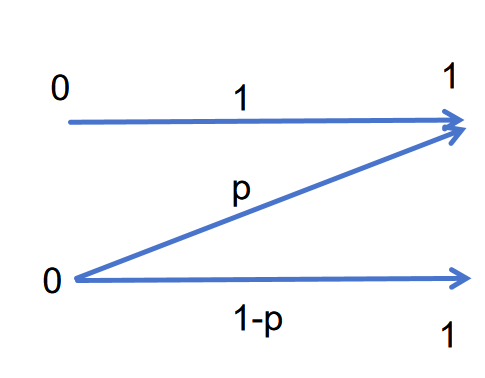
\includegraphics[width=0.2\linewidth]{4.png}
\end{center}


\tcblower

   信道矩阵为 $ \left(\begin{array}{cc}1 & 0 \\ p & 1-p\end{array}\right) $.
设入口分布为 $ \left(p_{0}, p_{1}\right) $ ,对应的出口分布为 $ \left(q_{0}, q_{1}\right) $,则 
$$ \left(q_{0}, q_{1}\right)=\left(p_{0}, p_{1}\right)\left(\begin{array}{cc}1 & 0 \\ p & 1-p\end{array}\right)=\left(p_{0}+p_{1} p, p_{1}(1-p)\right) $$
$$
\begin{aligned}
c & =\sum_{j=1}^{b} p\left(v_{j} \mid v_{i}\right) \log \frac{p\left(v_{j} \mid u_{i}\right)}{q\left(v_{j}\right)} \\
& =1 \cdot \log \frac{1}{q_{0}} \\
& =p \cdot \log \frac{p}{q_{0}}+(1-p) \log \frac{1-p}{q_{1}}
\end{aligned}
$$

根据等式有 $ -\log q_{0}=p \cdot \log \frac{p}{q_{0}}+(1-p) \cdot \log \frac{1-p}{q_{1}} $
$$
\begin{aligned}
-\log q_{0} & =p \log p-p \log q_{0}+(1-p) \log (1-p)-(1-p) \log q_{1} \\
H(p) & =(1-p) \log \frac{q_{0}}{q_{1}}
\end{aligned}
$$

于是 $ \frac{q_{0}}{q_{1}}=e^{\frac{H(p)}{1-p}} $.
由于 $ q_{0}+q_{1}=1 $ ,所以 $ \frac{1-q_{1}}{q_{1}}=e^{\frac{H(p)}{1-p}} $, 令 $ \lambda=\frac{H(p)}{1-p} $
解得 $ q_{1}=\frac{1}{1+e^{\lambda}} $, 则 $ q_{0}=\frac{e^{\lambda}}{1+e^{\lambda}} $
$$
\begin{aligned}
C=\log \frac{1}{q_{0}}=\log \frac{1+e^{\lambda}}{e^{\lambda}} & =\log \left(1+\frac{1}{e^{\lambda}}\right) \\
& =\log \left(1+e^{-\frac{H(p)}{1-p}}\right)
\end{aligned}
$$
    
\end{tcolorbox}